\chapter{Исследовательская часть}

В данном разделе приведены примеры работы программ, постановка эксперимента и сравнительный анализ алгоритмов на основе полученных данных.

\section{Технические характеристики}

Технические характеристики устройства, на котором выполнялось исследование, следующие.

\begin{enumerate}
	\item Операционная система: Windows 10 Корпоративная, Версия	21H1, Сборка ОС 19043.2006.
	\item Оперативная память: 8 ГБ.
	\item Процессор: AMD Ryzen 5 4600H с видеокартой Radeon Graphics \\3.00 ГГц \cite{processor}.
\end{enumerate}

Исследование проводилось на ноутбуке, включенном в сеть электропитания. 
Во время исследования ноутбук был нагружен только операционной системой и фоновыми приложениями.

\section{Демонстрация работы программы}

На рисунках \ref{fig:demographics}, \ref{fig:smoke}, \ref{fig:democonsole}, представлены результат работы реализации алгоритма обратной трассировки лучей.

\captionsetup{justification=centering, singlelinecheck=false}
\begin{figure}[H]
	\centering
	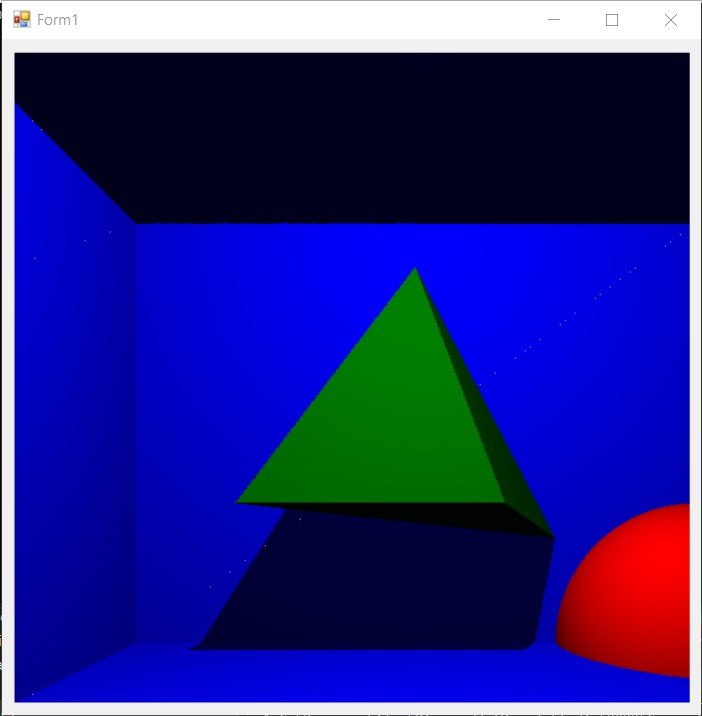
\includegraphics[width=1\linewidth]{inc/img/demographics}
	\caption{Демонстрация работы программы в графическом интерфейсе без дыма}
	\label{fig:demographics}
\end{figure}
\begin{figure}[H]
	\centering
	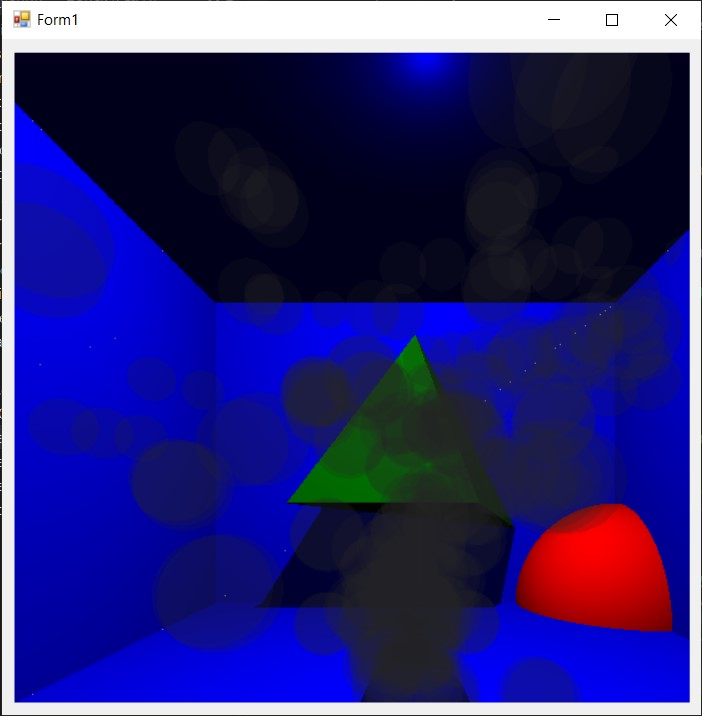
\includegraphics{inc/img/smoke}
	\caption{Демонстрация работы программы в графическом интерфейсе с дымом}
	\label{fig:smoke}
\end{figure}


\begin{figure}[H]
	\centering
	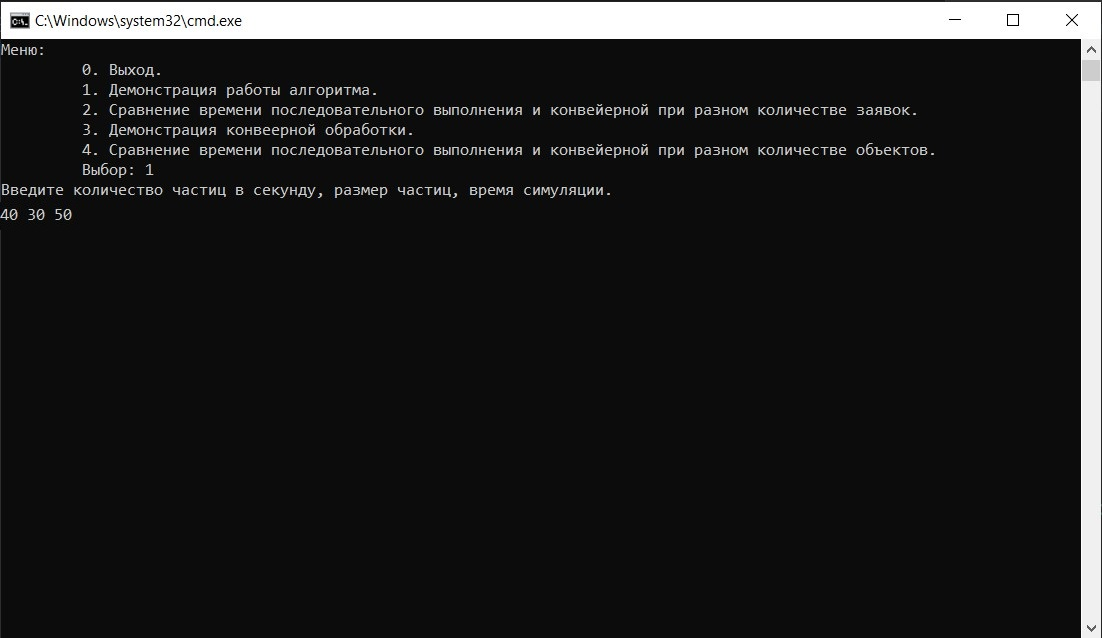
\includegraphics[width=1\linewidth]{inc/img/democonsole}
	\caption{Демонстрация работы программы в консоли}
	\label{fig:democonsole}
\end{figure}

Пример лог-файла приведен в приложении А.

\section{Сравнение времени работы реализаций последовательного алгоритма и конвейерного при разном количестве пикселей}

Замеры времени для каждого количества заявок проводились 50 раз. 
В качестве результата взято среднее время работы алгоритма на данном количестве заявок.
Результаты замеров времени (секунды) приведены в таблице \ref{tab:single}.
На рисунке \ref{fig:queries}, приведена зависимость времени работы реализаций алгоритмов при последовательном и конвейерном выполнении от количества заявок`. 

\captionsetup{justification=raggedright, singlelinecheck=false}
\begin{table}[H]
	\begin{center}
\begin{threeparttable}
		
		\caption{\label{tab:single}Время выполнения реализаций алгоритма обратной трассировки лучей при конвейерном и последовательном выполнении}
		\begin{tabular}{|c|d|d|}
			\hline
			Количество пикселей & \multicolumn{1}{c|}{Последовательное}  &  \multicolumn{1}{c|}{Конвейерное} \\\hline
			38400&	18.561&	16.652 \\\hline
			76800&	37.364&	33.513 \\\hline
			115200&	56.002&	50.518 \\\hline
			153600&	74.269&	67.199 \\\hline
			230400&	111.498&	101.034 \\\hline
			307200&	148.789&	135.163 \\\hline
			345600&	167.347&	152.163 \\\hline
			460800&	223.285&	202.800 \\\hline
		\end{tabular}
	\end{threeparttable}
	\end{center}
\end{table}
\captionsetup{justification=centering,singlelinecheck=false}
\begin{figure}[H]
	\centering
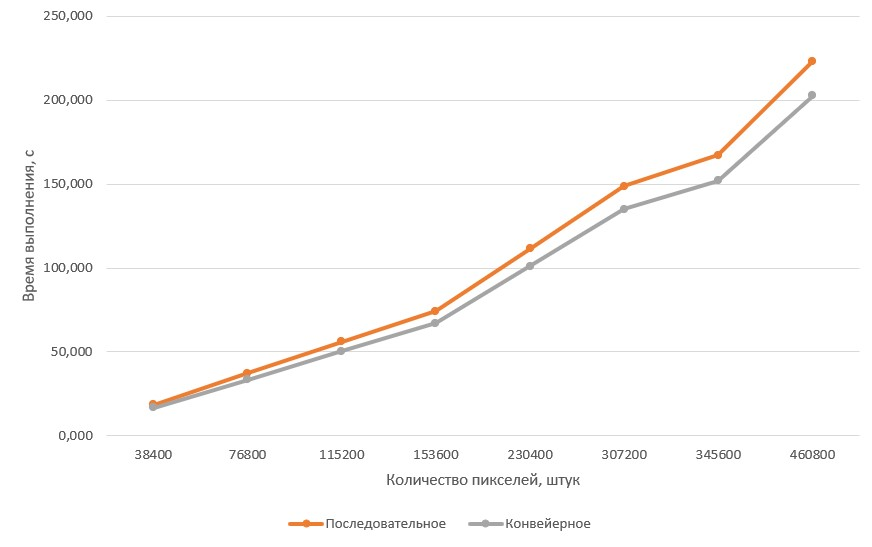
\includegraphics[width=0.9\linewidth]{inc/img/queries}
	\caption{Зависимость времени выполнения реализаций алгоритма обратной трассировки лучей при конвейерном и последовательном выполнении от количества пикселей}
	\label{fig:queries}
\end{figure}

Конвейерная реализация работает быстрее, чем последовательная на 10 -- 12\%.

\section{Сравнение времени работы реализаций последовательного алгоритма и конвейерного при разном количестве объектов на сцене}

Замеры времени для каждого количества объектов проводились 50 раз. 
В качестве результата взято среднее время работы реализации алгоритма на данном количестве объектов.
Под объектом понимается отдельная поверхность, т.е. плоскость полигона или сфера.
Результаты замеров времени (секунды) приведены в таблице \ref{tab:time}.
На рисунке \ref{fig:objects} приведена зависимость времени работы реализаций алгоритмов при последовательном и конвейерном исполнении от количества объектов на сцене.
\captionsetup{justification=raggedright,singlelinecheck=false}
\begin{table}[H]
	\begin{center}
	\begin{threeparttable}
		\caption{\label{tab:time}Время выполнения реализаций алгоритмов при последовательном и конвейерном выполнении от количества объектов на сцене}
		\begin{tabular}{|c|d|d|}
			\hline				
			Количество объектов &  \multicolumn{1}{c|}{Последовательный}  &  \multicolumn{1}{c|}{Конвейерный} \\\hline
			4&0.7596&0.8106\\\hline
			104&0.8134&0.8158\\\hline
			204&0.8676&0.8624\\\hline
			304&0.9214&0.8768\\\hline
			404&0.9694&0.901\\\hline
			504&1.0156&0.9428\\\hline
			604&1.0656&0.9596\\\hline
			704&1.1096&0.9704\\\hline
			804&1.1554&1.012\\\hline
			904&1.2014&1.0124\\\hline
		\end{tabular}
	\end{threeparttable}
	\end{center}
\end{table}
\captionsetup{justification=centering,singlelinecheck=false}

\begin{figure}[H]
	\centering
	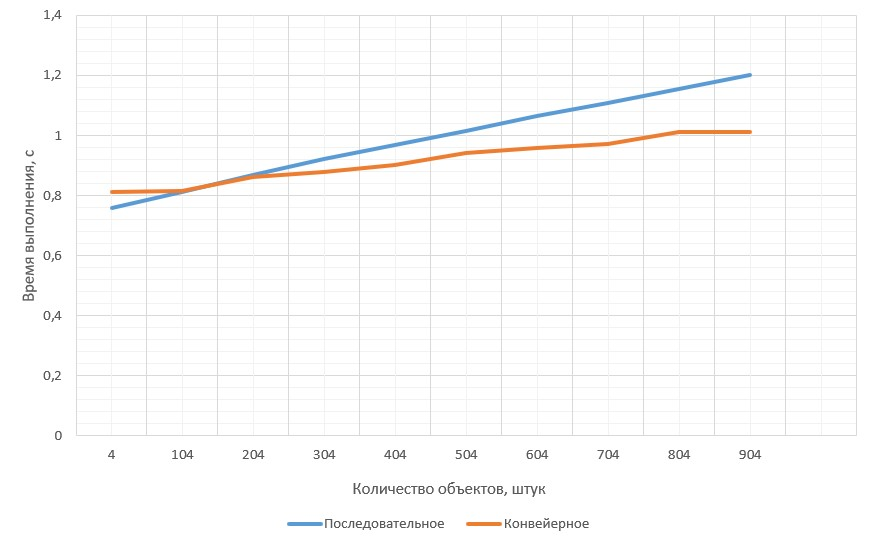
\includegraphics[width=0.9\linewidth]{inc/img/objects}
	\caption{Зависимость времени работы реализаций алгоритмов при последовательном и конвейерном выполнении от количества объектов на сцене}
	\label{fig:objects}
\end{figure}

Реализация последовательного алгоритма работает быстрее реализации конвейерного, если объектов на сцене меньше, чем 104. 
Это объясняется тем, что время, затраченное на создание потоков конвейерных линий, их обслуживание и перекладывание заявок из очереди в очередь превышает время, выигранное при параллельной обработке.

\section*{Вывод}

В данном разделе было произведено сравнение времени выполнения реализации алгоритма трассировки лучей при последовательной реализации и конвейерной.
Результат показал, что если объектов на сцене меньше, чем 104, то последовательная реализация эффективнее по времени, чем конвейерная.

